\documentclass{article}
\usepackage{amsthm}
\usepackage{amsmath}
\usepackage{amssymb}
\usepackage{amsfonts}
\usepackage{graphicx}
\usepackage{wrapfig}
\usepackage{tabu}
\usepackage{hyperref}
\usepackage{booktabs}
\usepackage{listings}
\graphicspath{ {./Images/} }

\makeatletter
\def\lecture{\@ifnextchar[{\@lectureWith}{\@lectureWithout}}
\def\@lectureWith[#1]{\medbreak\refstepcounter{section}%
	\renewcommand{\leftmark}{Lecture \thesection}
	\noindent{\addcontentsline{toc}{section}{Lecture \thesection: #1\@addpunct{.}}%
		\sectionfont Lecture \thesection. #1\@addpunct{.}}\medbreak}
\def\@lectureWithout{\medbreak\refstepcounter{section}%
	\renewcommand{\leftmark}{Lecture \thesection}
	\noindent{\addcontentsline{toc}{section}{Lecture \thesection.}%
		\sectionfont Lecture \thesection.}\medbreak}
\makeatother

\newcommand{\n}{\newline}

\title{CMSC 660 HW I}
\date{9/3/18}
\author{Joe Asercion}
\begin{document}
	\maketitle
	\section{Chapter 2, Problem 3}
		\subsection{Proof}
		Show that $f_{j,k}=\sin(x_{0}+(j-k)\frac{\pi}{3})$ satisfies the recurrence relation
		\begin{center}
			$f_{j,k+1}=f_{j,k}-f_{j+1,k}$
		\end{center}
		
		\subsubsection{Answer}
		
		Applying the trigonometric identity\n
		\begin{equation}
			\begin{split}
				\sin(\alpha\pm\beta)&=\sin(\alpha)\cos(\beta)\pm\cos(\alpha)\sin(\beta)
			\end{split}
		\end{equation}
		Allows  $f_{j+1,k}$ to be written as:
		\begin{equation}
			\begin{split}
				f_{j+1,k}&=\sin(x_{0}+(j+1-k)\frac{\pi}{3}) \\
				&=\sin(x_{0}+(j-k)\frac{\pi}{3}+\frac{\pi}{3}))\\
				&=\sin(\frac{\pi}{3})\cos(x_{0}+(j-k)\frac{\pi}{3})+\cos(\frac{\pi}{3})\sin(x_{0}+(j-k)\frac{\pi}{3})\\
				&=\frac{\sqrt{3}}{2}\cos(x_{0}+(j-k)\frac{\pi}{3})+\frac{1}{2}\sin(x_{0}+(j-k)\frac{\pi}{3})
			\end{split}
		\end{equation}
		
		Therefore we can write the $f_{j,k}-f_{j+1,k}$ as 
		\begin{equation}
			\begin{split}
			f_{j,k}-f_{j+1,k} &= \sin(x_{0}+(j-k)\frac{\pi}{3})-(\frac{\sqrt{3}}{2}\cos(x_{0}+(j-k)\frac{\pi}{3})+\frac{1}{2}\sin(x_{0}+(j-k)\frac{\pi}{3})) \\
			&=\frac{1}{2}\sin(x_{0}+(j-k)\frac{\pi}{3})-\frac{\sqrt{3}}{2}\cos(x_{0}+(j-k)\frac{\pi}{3})
			\end{split}
		\end{equation}
		
		Applying the same trigonometric identity to $f_{j,k+1}$ yields
		\begin{equation}
			\begin{split}
			f_{j,k+1} &= \sin(x_{0}+(j-k-1)\frac{\pi}{3}) \\
			&=\sin(x_{0}+(j-k)\frac{\pi}{3}-\frac{\pi}{3}) \\
			&=\sin(-\frac{\pi}{3})\cos(x_{0}+(j-k)\frac{\pi}{3})+\cos(-\frac{\pi}{3})\sin(x_{0}+(j-k)\frac{\pi}{3})\\
			&=-\frac{\sqrt{3}}{2}\cos(x_{0}+(j-k)\frac{\pi}{3})+\frac{1}{2}\sin(x_{0}+(j-k)\frac{\pi}{3})
			\end{split}
		\end{equation}
		
		We therefore see
		
		\begin{equation}
			\begin{split}
			f_{j,k+1} &= -\frac{\sqrt{3}}{2}\cos(x_{0}+(j-k)\frac{\pi}{3})+\frac{1}{2}\sin(x_{0}+(j-k)\frac{\pi}{3})\\
			f_{j,k}-f_{j+1,k}&=\frac{1}{2}\sin(x_{0}+(j-k)\frac{\pi}{3})-\frac{\sqrt{3}}{2}\cos(x_{0}+(j-k)\frac{\pi}{3})\\
			\therefore f_{j,k+1} &=f_{j,k}-f_{j+1,k}
			\end{split}
		\end{equation}
		
		\subsection{Proof}
		Show that if $|\hat{f}_{j,k}-f_{j,k}|\leq\epsilon$ for all $j$ then $|\hat{f}_{j,k+1}-f_{j,k+1}|\leq2\epsilon$ for all $j$.
		
		\subsubsection{Answer}
		We know from the recurrence relation $f_{j,k+1}=f_{j,k}-f_{j+1,k}$ that we can rewrite the second expression: 
		
		\begin{equation}
			\begin{split}
			|\hat{f}_{j,k+1}-f_{j,k+1}| &= |(\hat{f}_{j,k}-\hat{f}_{j+1,k})-(f_{j,k}-f_{j+1,k})| \\
			&=|(\hat{f}_{j,k}-f_{j,k})+(f_{j+1,k}-\hat{f}_{j+1,k})| \\
			&= |\hat{f}_{j,k}-f_{j,k}|+|f_{j+1,k}-\hat{f}_{j+1,k}|\\
			&=|\hat{f}_{j,k}-f_{j,k}|+|\hat{f}_{j+1,k}-f_{j+1,k}|
			\end{split}
		\end{equation}
	
		We are given the relation $|\hat{f}_{j,k}-f_{j,k}|\leq\epsilon$ for all $j$.  Therefore we can state 
		
		\begin{equation}
			\begin{split}
			|\hat{f}_{j,k}-f_{j,k}|+|\hat{f}_{j+1,k}-f_{j+1,k}| \leq\epsilon+|\hat{f}_{j+1,k}-f_{j+1,k}|		
			\end{split}
		\end{equation}
		
		Since the relation applies for all $j$, we can state
		
		\begin{equation}
			\begin{split}
			|\hat{f}_{j+1,k}-f_{j+1,k}|\leq\epsilon
			\end{split}
		\end{equation}
		
		Therefore,
		
		\begin{equation}
			\begin{split}
			|\hat{f}_{j,k}-f_{j,k}|+|\hat{f}_{j+1,k}-f_{j+1,k}|&\leq\epsilon+\epsilon\\
			|\hat{f}_{j,k}-f_{j,k}|+|\hat{f}_{j+1,k}-f_{j+1,k}|&\leq2\epsilon\\
			\therefore |\hat{f}_{j,k+1}-f_{j,k+1}| \leq2\epsilon
			\end{split}
		\end{equation}
		
		\subsection{Code}
		Write a program that computes $e_{k}=\hat{f_{0,k}}-f_{0,k}$ for $1\leq k\leq60$ and $x_{0}=1$.  Print the $e_{k}$ and see whether they grow monotonically.  Plot the $e_{k}$ on a linear scale and note what happens around $k=50$.  Plot the $e_{k}$ on a log scale.  For comparison, include a straight line that would represent the error if it were exactly to double each time.
		
		\subsubsection{Answer}
		All code is attached in an appendix.  Plots and tables below.\n		
		\newpage
		\textbf{$\epsilon_{k}$ Table: \n}
		\begin{center}
		\resizebox{!}{.4\textheight}{
			\begin{tabular}{c}
				$\epsilon_{k}$, $k=[1,60]$ \\
				\toprule
				-2.91433543964104e-16\\
				-2.22044604925031e-16\\
				-1.11022302462516e-16\\
				1.94289029309402e-16\\
				-2.22044604925031e-16\\
				-3.33066907387547e-16\\
				-5.34294830600857e-16\\
				-3.33066907387547e-16\\
				-4.44089209850063e-16\\
				-7.84095011141517e-16\\
				1.11022302462516e-16\\
				4.44089209850063e-16\\
				7.70217223333702e-16\\
				-1.11022302462516e-16\\
				6.66133814775094e-16\\
				-3.19189119579733e-16\\
				-1.22124532708767e-15\\
				-1.33226762955019e-15\\
				-1.91513471747840e-15\\
				2.22044604925031e-16\\
				7.77156117237610e-16\\
				1.58900670399476e-15\\
				1.22124532708767e-15\\
				1.88737914186277e-15\\
				3.39311911901063e-15\\
				1.11022302462516e-15\\
				1.22124532708767e-15\\
				1.83880688453542e-15\\
				-2.22044604925031e-16\\
				-2.77555756156289e-15\\
				9.29811783123569e-16\\
				0\\
				-3.21964677141295e-15\\
				-3.60822483003176e-16\\
				4.44089209850063e-16\\
				-5.55111512312578e-16\\
				-1.42247325030098e-15\\
				-1.22124532708767e-15\\
				1.11022302462516e-16\\
				-5.77315972805081e-15\\
				8.88178419700125e-16\\
				3.55271367880050e-15\\
				4.37150315946155e-16\\
				-3.33066907387547e-16\\
				-3.33066907387547e-15\\
				6.67521593555875e-15\\
				6.66133814775094e-16\\
				-3.33066907387547e-16\\
				-1.36002320516582e-15\\
				2.10942374678780e-15\\
				5.55111512312578e-15\\
				-3.17801340798951e-15\\
				-9.99200722162641e-16\\
				-1.22124532708767e-15\\
				5.27355936696949e-15\\
				-1.22124532708767e-15\\
				1.11022302462516e-16\\
				-5.82173198537817e-15\\
				-2.33146835171283e-15\\
				-5.66213742558830e-15
			\end{tabular}
		}
		\newpage
		\textbf{Linear Plot: \n}
		\resizebox{.9\textwidth}{!}{
			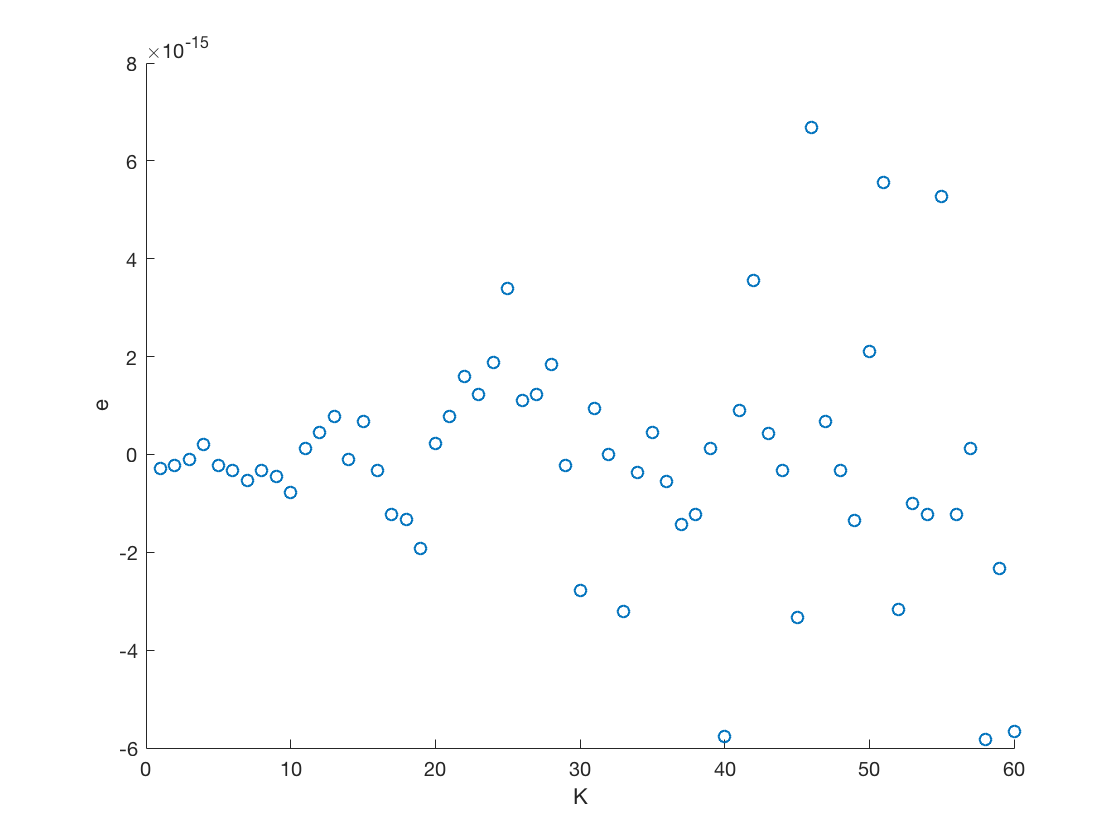
\includegraphics{Prob1_Linear.png}
		}
		
		\textbf{Log Plot: \n}
		
		\resizebox{.9\textwidth}{!}{
			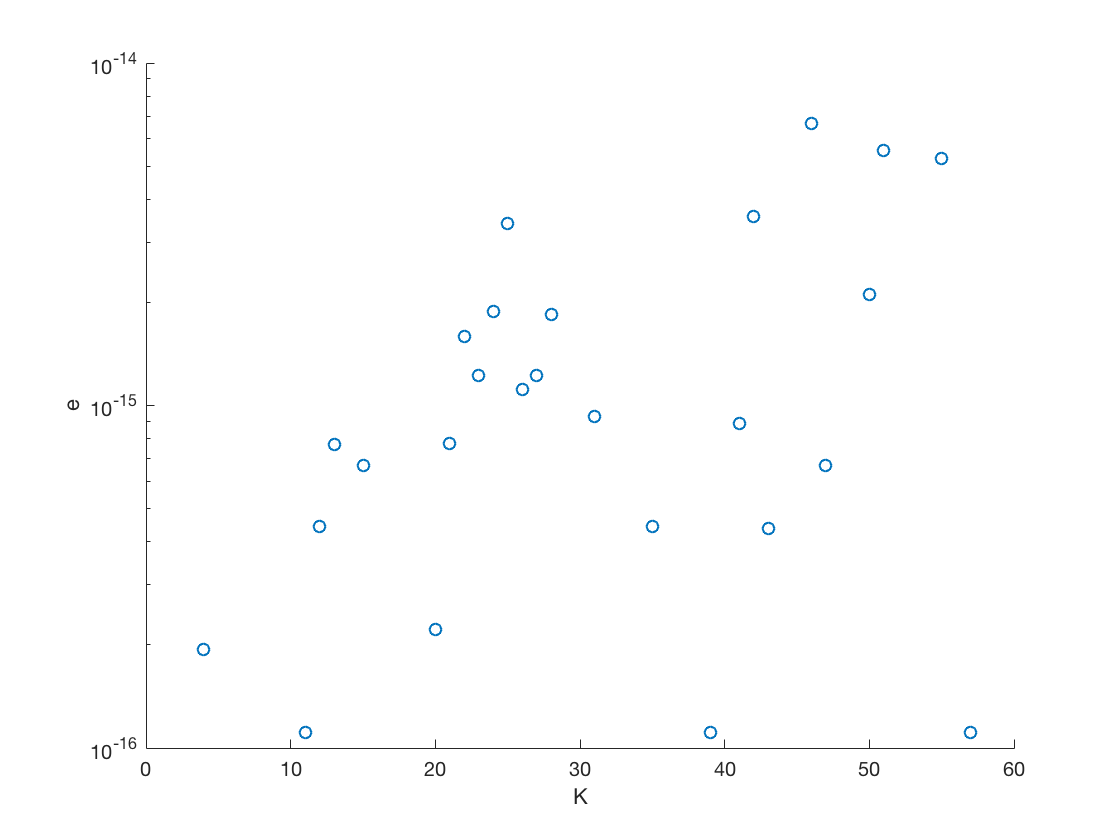
\includegraphics{Prob1_Log.png}
		}
	\end{center}
	\section{Chapter 2, Problem 7}
	
	\subsection{a. Arithmetic}
	Do these two expressions result in the same floating point number (down to the last bit) as long as no NaN or inf values or denormalized numbers are produced? \n
	
	\begin{flushleft}
	\begin{math}
		(x*y)+(z-w)\n
		(z-w)+(y*x)
	\end{math}
	\end{flushleft}
	
	\subsubsection{Answer}
	From Bindle and Goodman pg.10, we know that floating point addition and multiplication following the IEEE standard for arithmetic operation is commutative.  Therefore, we can can state
	
	\begin{equation}
		\begin{split}
		(x*y)+(z-w)=(x*y)+(z-w)
		\end{split}
	\end{equation}
	
	So long as floating point calculation produces no underflow or overflow exception, both of these expressions will return the same floating point number down to the last bit. 
	
	\subsection{b. Arithmetic}
	Do these two expressions result in the same floating point number (down to the last bit) as long as no NaN or inf values or denormalized numbers are produced? \n
	
	\begin{flushleft}
	\begin{math}
	(x+y)+z\n
	x+(y+z)
	\end{math}
	\end{flushleft}
	
	\subsubsection{Answer}
	This operation is susceptible to rounding error.  Modeling the error of the first expression yields:
	
	\begin{equation}
		\begin{split}
		fl((x+y)+z)&=((x+y)(1+\epsilon_{1})+z)(1+\epsilon_{2})\\
		&=(x+x\epsilon_{1}+y+y\epsilon_{1}+z)(1+\epsilon_{2})\\
		&=(x+y+z+x\epsilon_{1}+y\epsilon_{1})(1+\epsilon_{2})\\
		&=x+y+z+x\epsilon_{1}+y\epsilon_{1}+x\epsilon_{2}+y\epsilon_{2}+z\epsilon_{2}+x\epsilon_{1}\epsilon_{2}+y\epsilon_{1}\epsilon_{2}\\
		&=(x+y+z)+(x+y)\epsilon_{1}+(x+y+z)\epsilon_{2}+(x+y)\epsilon_{1}\epsilon_{2}
		\end{split}
	\end{equation}
	
	As noted on Bindle and Goodman pg. 11, we can drop the mixed $\epsilon$ term as it will be smaller than either $\epsilon_{1}$ or $\epsilon_{2}$ by a factor of $\epsilon_{mach}$.  This is true because $|\epsilon|\leq\epsilon_{mach}$ (B\&G pg.10).  Therefore we can state
	
	\begin{equation}
		\begin{split}
		fl((x+y)+z)\approx(x+y+z)+(x+y)\epsilon_{1}+(x+y+z)\epsilon_{2}
		\end{split}
	\end{equation}
	
	Performing the same error estimation on the second expression yields:
	
	\begin{equation}
		\begin{split}
		fl(x+(y+z))&=(y+z)+x \text{ since, as previously stated, floating point addition is commutative }\\
		&=((y+z)(1+\epsilon_{1'})+x)(1+\epsilon_{2'})\\
		&=(y+z+y\epsilon_{1'}+z\epsilon_{1'}+x)(1+\epsilon_{2'})\\
		&=(x+y+z)+(y+z)\epsilon_{1'}+(x+y+z)\epsilon_{2'}+(y+z)\epsilon_{1'}\epsilon_{2'}
		\end{split}
	\end{equation}
	
	We again drop the mixed term for the reason stated above and write:
	
	\begin{equation}
		\begin{split}
		fl(x+(y+z))\approx(x+y+z)+(y+z)\epsilon_{1'}+(x+y+z)\epsilon_{2'}
		\end{split}
	\end{equation}
	
	Comparing equation (12) and (14) shows that, in fact, $fl(x+(y+z))$ does not necessarily yield the same bitwise result as $fl((x+y)+z)$.  Therefore, floating point addition is not associative.
	
	  
	
	\subsection{c. Arithmetic}
	Do these two expressions result in the same floating point number (down to the last bit) as long as no NaN or inf values or denormalized numbers are produced? \n
	
	\begin{flushleft}
	\begin{math}
	x*\text{oneHalf}+y*\text{oneHalf}\n
	(x+y)*\text{oneHalf}
	\end{math}
	\end{flushleft}
	
	\subsubsection{Answer}
	From B\&G pg. 11, we know that division by powers of 2 is exact so long as the result is a normalized number.  Therefore, the only error introduced in these expressions is due to rounding in the floating point addition step.  Starting with the first expression,
	
	\begin{equation}
		\begin{split}
		&fl(x*\text{oneHalf}+y*\text{oneHalf})=(x*\text{oneHalf}+y*\text{oneHalf})(1+\epsilon_{1})\\
		&=(x*\text{oneHalf}+y*\text{oneHalf})+(x*\text{oneHalf}+y*\text{oneHalf})\epsilon_{1}
		\end{split}
	\end{equation}
	
	Because division by 2 is exact, we can rewrite the above expression as
	
	\begin{equation}
		\begin{split}
		fl(x*\text{oneHalf}+y*\text{oneHalf})=((x+y)+(x+y)(\epsilon_{1}))*\text{oneHalf}
		\end{split}
	\end{equation}
	
	Doing the same for the second expression yields
	
	\begin{equation}
		\begin{split}
		&fl((x+y)*\text{oneHalf})=(x+y)(1+\epsilon_{1'})*\text{oneHalf}\\
		&fl((x+y)*\text{oneHalf})=((x+y)+(x+y)(\epsilon_{1'}))*\text{oneHalf}
		\end{split}
	\end{equation}
	
	Comparing the results in equations (17) and (16) shows that both expressions yield the same bitwise floating point number.
	
	\subsection{d. Arithmetic}
	Do these two expressions result in the same floating point number (down to the last bit) as long as no NaN or inf values or denormalized numbers are produced? \n
	
	\begin{flushleft}
	\begin{math}
	x*\text{oneThird}+y*\text{oneThird}\n
	(x+y)*\text{oneThird}
	\end{math}
	\end{flushleft}
	
	\subsubsection{Answer}
	
	As noted in part c, division by three must not be exact as 3 is not a power of 2.  Because we know from part b that floating point addition is not associative and division by 3 introduces its own error we can immediately come to the conclusion that these two expressions will not produce the same bitwise floating point number.
	
	\section{Chapter 2, Problem 6}
	
	\subsection{Proof}
	Show that the absolute error in the Sum $S$ computed by the code in the text is no worse than $(n-1)\epsilon_{mach}\sum^{n-1}_{k=0} |x_{i}|$ if the floating point sum $x+y$ has relative error $\epsilon<\epsilon_{mach}$.
	
	\subsubsection{Answer}
	
	Performing the error analysis and expanding the summation function out yields:
	
	\begin{equation}
		\begin{split}
		fl(\sum_{i=0}^{n-1}x[i])&=(((x[0]+x[1])(1+\epsilon_{0})+x[2])(1+\epsilon_{1})+x[3])(1+\epsilon_{3})+...\\
		&\approx((x[0]+x[1])+(x[0]+x[1])\epsilon_{0}+(x[0]+x[1]+x[2])+(x[0]+x[1]+x[2])\epsilon_{1}+...
		\end{split}
	\end{equation}
	
	Noting that in this case the array containing the summation terms is indexed at zero.  Above we also neglect error cross terms in the expansion, as those errors will be much smaller that the individual addition operation errors (as noted in previous problems).
	
	We can express the absolute error of this operation as:
	
	\begin{equation}
		\begin{split}
		(\sum^{n-1}_{i=0}\epsilon_{i})(\sum^{n-1}_{i=0}|x_{i}|)
		\end{split}
	\end{equation}   
	There are a total of $n-1$ error values in the operation, as each term in the summation contribute one $\epsilon$ value except for $x[0]$.
	
	The largest error contribution in the summation will be provided by the largest $\epsilon$ value due to a summation operation in the above expansion.  Therefore, if we let $\epsilon_{largest}$ represent the largest $\epsilon_{i}$ value we can write
	
	\begin{equation}
		\begin{split}
		\sum^{n-1}_{i=0}\epsilon_{i}\leq(n-1)\epsilon_{largest}
		\end{split}
	\end{equation}
	
	From B\&G pg 10, we know that any individual error value is upper bounded by the machine precision.  i.e. $|\epsilon|\leq\epsilon_{mach}$.  Therefore, we can state
	
	\begin{equation}
		\begin{split}
		(n-1)\epsilon_{largest}\leq(n-1)\epsilon_{mach}
		\end{split}
	\end{equation}
	
	Which implies
	
	\begin{equation}
		\begin{split}
		(\sum^{n-1}_{i=0}\epsilon_{i})(\sum^{n-1}_{i=0}|x_{i}|)\leq(n-1)\epsilon_{mach}\sum^{n-1}_{i=0}|x_{i}|
		\end{split}
	\end{equation}
	
	\section{Chapter 2, Problem 9}
	\subsection{a. Code}
	Using the recurrence relation $a_{n,k+1}=\frac{n-k}{k+1}a_{n,k}$, compute $a_{n,k}$ for a range of $n$ values.
	
	\subsubsection{Answer}
	
	Code found in the appendix.  Computed values for $n=[1,10]$ below.  Computations run from $a_{n,0}$ to $a_{n,n+1}$ for each value $n$.\n
	\begin{center}
		\newpage
		\textbf{Single Precision Computed Values\n}
	\end{center}
	
	\resizebox{\textwidth}{!}{
		\begin{tabular}{c|c|c|c|c|c|c|c|c|c}
			n=1 & n=2 & n=3 & n=4 & n=5 & n=6 & n=7 & n=8 & n=9 & n=10 \\
			1&1&1&1&1&1&1&1&1&1 \\
			0&0.5&1&1.5&2&2.5&3&3.5&4&4.5 \\
			&0&0.333333343267441&1&2&3.33333325386047&5&7&9.33333301544189&12 \\
			&&0&0.25&1&2.5&5&8.75&14&21 \\
			&&&0&0.200000002980232&1&3&7&14&25.2000007629395 \\
			&&&&0&0.16666667163372&1&3.5&9.33333301544189&21 \\
			&&&&&0&0.142857149243355&1&3.99999976158142&12 \\
			&&&&&&0&0.125&0.999999940395355&4.5 \\
			&&&&&&&0&0.111111104488373&1 \\
			&&&&&&&&0&0.100000001490116 \\
			&&&&&&&&&0			
		\end{tabular}
	}	
	\begin{center}
		\textbf{\n Double Precision Computed Values\n}
	\end{center}
	\resizebox{\textwidth}{!}{
		\begin{tabular}{c|c|c|c|c|c|c|c|c|c}
			n=1 & n=2 & n=3 & n=4 & n=5 & n=6 & n=7 & n=8 & n=9 & n=10 \\
			1&1&1&1&1&1&1&1&1&1\\
			0&0.5&1&1.5&2&2.5&3&3.5&4&4.5\\
			&0&0.333333333333333&1&2&3.33333333333333&5&7&9.33333333333333&12\\
			&&0&0.25&1&2.5&5&8.75&14&21\\
			&&&0&0.2&1&3&7&14&25.2\\
			&&&&0&0.166666666666667&1&3.5&9.33333333333333&21\\
			&&&&&0&0.142857142857143&1&4&12\\
			&&&&&&0&0.125&1&4.5\\
			&&&&&&&0&0.111111111111111&1\\
			&&&&&&&&0&0.1\\
			&&&&&&&&&0
		\end{tabular}
	}
	
	\subsection{a.  Reasoning}
	Why is roundoff not a problem here?  Comparing values where $\hat{a_{n,n}}\approx1$ in double precision but not in single precision explain how this is possible given roundoff not being a problem.
	
	\subsubsection{Answer}
	
	The value of $n$ for which the calculated $\hat{a}_{n,n}\approx1$ in double precision but not single precision in this range is \n
	
	$n=9$\n
	\begin{flushleft}
		\textbf{Single Precision: }.999999940395355\n
		\textbf{Double Precision: }1\n
	\end{flushleft}
	
	\subsection{b.  Code}
	Use the algorithm from part a to compute:\n
	
	\begin{flushleft}
		\begin{math}
		E(k)=\frac{1}{2^{n}}\sum^{n}_{k=0}ka_{n,k}=\frac{n}{2}
		\end{math}
	\end{flushleft}
	Do not safeguard against overflow or zero divide.  Show in both single and double precision that the computed answer has high accuracy as long as the intermediate results are within the range of floating point numbers.
	
	\subsubsection{Answer}
	Code is in the appendix.  Calculated values for $n=[1,10]$ in both single and double precision:
	
	\begin{center}
		\textbf{Single Precision Computed Values\n}
	\end{center}
	
	\resizebox{\textwidth}{!}{
		\begin{tabular}{c|c|c|c|c|c|c|c|c|c}
			n=1 & n=2 & n=3 & n=4 & n=5 & n=6 & n=7 & n=8 & n=9 & n=10 \\
			0&0.125&0.208333343267441&0.265625&0.306250005960464&0.3359375&0.358258932828903&0.37548828125&0.389105886220932&0.400097638368607 
		\end{tabular}
	}		

	\begin{center}
		\textbf{Double Precision Computed Values\n}
	\end{center}
	
	\resizebox{\textwidth}{!}{
		\begin{tabular}{c|c|c|c|c|c|c|c|c|c}
			n=1 & n=2 & n=3 & n=4 & n=5 & n=6 & n=7 & n=8 & n=9 & n=10 \\
			0&0.125&0.208333333333333&0.265625&0.30625&0.3359375&0.358258928571429&0.37548828125&0.389105902777778&0.40009765625 
		\end{tabular}
	}		
	
	
	\subsection{b. Reasoning}
	Explain how the computer gets an accurate, small answer when the intermediate numbers have such a wide range of values.  Why is cancellation not a problem?
	
	\subsubsection{Answer}

	%\subsection{b. Code}
	%Print $E(k)$ as computed by the formula in part b and $M_{n}=max_{k}a_{n,k}$.
	
	%\subsubsection{Answer}
	
	%\subsection{b. Reasoning}
	%For large $n$, one should be inf and the other NaN.  Explain why.
	
	%\subsubsection{Answer}
	
	\section{Code Appendix}
	
	\subsection{Problem 1}
	
	\begin{lstlisting}
	%*****************************
	% CMSC660 HW1 Problem 1
	% Joe Asercion
	%*****************************
	
	%Set used variables
	x=1;
	j=0;
	kmin = 1;
	kmax = 60;
	len = kmax-kmin;
	f1 = zeros(len,1);
	f2 = zeros(len,1);
	e = zeros(len,1);
	
	%Calculate approximation
	f1(1) = double(sin(x)-sin(x+pi/3));
	for k = kmin:kmax
	%Second term generated using trig identity
	%sin(a+b)=sin(a)cos(b)+cos(a)sin(b) in order to use the recursive f1(k)
	%term
	f1(k+1) = double(f1(k)-((sqrt(3)/2)*cos(x-k*pi/3)+(1/2)*f1(k)));
	%f1(k+1) = double(f1(k)-sin(x+(1-k)*pi/3));
	end
	
	%Calculate exact
	for k = kmin:kmax
	f2(k)= sin(x-k*pi/3);
	end
	
	%Calculate absolute error
	for i = kmin:kmax
	e(i) = f1(i)-f2(i);
	end
	
	%Plot
	scatter(kmin:kmax,e);
	set(gca,'yscale','log');
	xlabel('K'); % x-axis label
	ylabel('e') % y-axis label
	\end{lstlisting}
	
	\subsection{Problem 4.a}
	
	\begin{lstlisting}
	%*****************************
	% CMSC660 HW1 Problem 4 Part a
	% Joe Asercion
	%*****************************
	
	
	%***********************
	%Single Precision Case
	%***********************
	
	% Range of 'n' to calculate over
	
	n=1:10;
	len=range(n);
	
	% Array to hold output values from loops
	singleArr=zeros(len,len);
	
	
	for j=(1:10) % Outer loop iterates over n values 
	for k=(0:j) % Inner loop iterates over k from 0 to the current n value
	if k == 0
	singleArr(k+1,j)=single(1); % k=0 case
	else
	singleArr(k+1,j)=single(singleArr(k,j)*(j-k)/(k+1)); % Recurrance relation calculation
	end
	end 
	end
	
	SingleT = array2table(singleArr);
	writetable(SingleT,'SingleTable.txt');
	%***********************
	%Double Precision Case
	%***********************
	
	% Range of 'n' to calculate over
	
	n=1:10;
	len=range(n);
	
	% Array to hold output values from loops
	doubleArr=zeros(len,len);
	
	
	for j=(1:10) % Outer loop iterates over n values 
	for k=(0:j) % Inner loop iterates over k from 0 to the current n value
	if k == 0
	doubleArr(k+1,j)=double(1); % k=0 case
	else
	doubleArr(k+1,j)=double(doubleArr(k,j)*(j-k)/(k+1)); % Recurrance relation calculation
	end
	end 
	end
	
	DoubleT = array2table(doubleArr);
	writetable(DoubleT,'DoubleTable.txt');
	\end{lstlisting}
	
	\subsection{Problem 4.b}
	\begin{lstlisting}
	%*****************************
	% CMSC660 HW1 Problem 4 Part b
	% Joe Asercion
	%*****************************
	
	
	%***********************
	%Single Precision Case
	%***********************
	
	% Range of 'n' to calculate over
	
	n=1:10;
	len=range(n);
	
	% Array to hold output values from loops
	kArr1=zeros(len,len);
	singleArr=zeros(len,1);
	sum1=0;
	
	
	for j=(1:10) % Outer loop iterates over n values 
	for k=(0:j) % Inner loop iterates over k from 0 to the current n value
	if k == 0
	kArr1(k+1,j)=single(1); % k=0 case
	else
	kArr1(k+1,j)=single(kArr1(k,j)*(j-k)/(k+1)); % Recurrance relation calculation
	end
	end
	for k=(0:j)
	sum1=single(sum1+k*kArr1(k+1,j));
	end
	singleArr(j)=single((1/(2^j))*sum1);
	sum1 = 0;
	end
	
	SingleT = array2table(singleArr);
	writetable(SingleT,'SingleTable.txt');
	%***********************
	%Double Precision Case
	%***********************
	
	% Range of 'n' to calculate over
	
	n=1:10;
	len=range(n);
	
	% Array to hold output values from loops
	doubleArr=zeros(len,1);
	kArr2=zeros(len,len);
	sum2=0;
	
	for j=(1:10) % Outer loop iterates over n values 
	for k=(0:j) % Inner loop iterates over k from 0 to the current n value
	if k == 0
	kArr2(k+1,j)=double(1); % k=0 case
	else
	kArr2(k+1,j)=double(kArr2(k,j)*(j-k)/(k+1)); % Recurrance relation calculation
	end
	end 
	for k=(0:j)
	sum2=double(sum2+k*kArr2(k+1,j));
	end
	doubleArr(j)=double((1/(2^j))*sum2);
	sum2 = 0;
	end
	
	DoubleT = array2table(doubleArr);
	writetable(DoubleT,'DoubleTable.txt');
	\end{lstlisting}
	
	
\end{document}